% ---- ETD Document Class and Useful Packages ---- %
\documentclass{ucetd}
\usepackage{subfigure,epsfig,amsfonts}
\usepackage{natbib}
\usepackage{amsmath}
\usepackage{amssymb}
\usepackage{amsthm}
% Add extra packages I need
\input{tex/preamble-custom}

%% Use these commands to set biographic information for the title page:
\title{Parent of Origin Effects on Gene Expression and Quantitative Traits in the Hutterites}
\author{Sahar Mozaffari}
\department{Genetics}
\division{Biological Sciences}
\degree{Doctor of Philosophy}
\date{2018}

%% Use these commands to set a dedication and epigraph text
\dedication{Dedication Text}
\epigraph{Epigraph Text}


\begin{document}
%% Basic setup commands
% If you don't want a title page comment out the next line and uncomment the line after it:
\maketitle
%\omittitle

% These lines can be commented out to disable the copyright/dedication/epigraph pages
\makecopyright
%\makededication
%\makeepigraph


%% Make the various tables of contents
\tableofcontents
\listoffigures
\listoftables

% Enter Acknowledgements here
% !TEX encoding = UTF-8 Unicode
\acknowledgments

I am truly grateful for the mentorship I received from my advisor, Carole Ober. I am very thankful for her support and guidance throughout the four years I have spent in her lab. 

I would also like to thank Dan Nicolae who constantly encouraged me to meet with him and helped me with statistical problems I never expected to encounter.

My committee has played an important role in my progress, and I am thankful for their advice and support. Yoav Gilad has always provided me with critical support that I have been greatly appreciative of. 

% Enter Abstract here
\abstract

Variants can affect traits differently depending on whether they are inherited from the mother or the father, but genome wide association studies (GWAS) treat maternal and paternal alleles as equivalent. In addition, the variants identified by GWAS do not account for a significant portion of the heritability for the corresponding trait and could be due to underlying biological mechanisms that are not yet well understood. My thesis addresses these limitations by disentangling the effects of maternal and paternal alleles on gene expression as well as on disease associated phenotypes in the Hutterites, a founder population of European descent. With phased genotype data we can ask questions about parent of origin effects in this population. First, I tested for maternal and paternal genetic associations on cardiovascular disease and asthma associated traits and developed a novel method to detect variants that have opposite effects on the trait of interest depending on the parent of origin of the variant. We identified variants that have maternal-only or paternal-only effects, as well as variants that have opposite effects on traits ? which would not be detected in a standard GWAS. this is the largest family based study of parent of origin effects on quantitative traits and the first to look for opposite parental effects. In the second chapter, I map RNA-seq from lymphoblastoid cell lines (LCLs) to parental haplotypes in 306  Hutterites and detect known imprinted genes and two novel imprinted genes (\emph{PXDC1} and \emph{PWAR6}) in known imprinted regions. These imprinting gene patterns are validated using parent of origin expression from peripheral blood leukocyte (PBL) RNA-seq from 99 different Hutterites; imprinting control regions near the novel genes are validated using PBL methylation in the same 99 Hutterites. Finally, I explore searching for parent of origin effects on gene expression, or parent of origin eQTLs, first for opposite effects and then maternal and paternal specific effects. 

\mainmatter
% Main body of text follows

% Chapter 01 - Introduction
\chapter{Introduction}

\section{Human Genetics and the Genetics of Complex Traits}

A central goal of genetics is to understand the contribution of genetic variation to phenotypic variation.


\begin{figure}
\centering
\includegraphics[width=5in]{img/ch01/fig-01-lowhangingfruit.pdf}
\caption[Low Hanging Fruit.]{\textbf{Asthma GWAS - low hanging fruit}}
\label{fig:lowhangingfruit}
\end{figure}


\section{On The Origin of Genomic Imprinting }

Genomic imprinting in its broadest sense suggests that a phenotype observed for a particular gene or genes depends on the sex of the parent from with the gamete containing that gene or genes originated \cite{Sapienza:1989vm}. It was said that a particular gene is imprinted if it results in a different phenotype when it is maternally inherited versus paternally inherited.

The first use of the term "imprinting" was used in reference to the recognition by the cell of of chromosomes in \textit{Sciara} \cite{Crouse:1960vc,Sapienza:1989vm}. "The "imprint" a chromosome bears is unrelated to the genic constitution of the chromosome and is determined only by the sex of the germ line through with the chromosome has been inherited." \cite{Crouse:1960vc} 

The preferential inactivation of the paternally-derived X chromosomes in mouse were the first demonstrations of a functional imprint in mammalian genomes \cite{Takagi:1975ua,Lyon:1984gh,Chandra:1975tb}. The first suggestion of imprinting on autosomes was by a deletion on mouse chromosome 17 that showed a different phenotype based on which parent the deletion was inherited from \cite{Johnson:1974uf,Johnson:1974kc}. The development of the pronuclear transplantation technique allowed for the creation of mice zygotes which contained only maternal or only paternal genetic contributions and provided evidence that the maternal and paternal genomes are not equal. The differential imprinting on the parental chromosomes prevented complete embryonic development in these mice with complete uniparental disomy \cite{Sapienza:1989vm,McGrath:1984ky}. 

Further experiments suggested that imprinting occurs during gametogenesis and is necessary for full term development; an egg with a male pronucleus developed to term, however, an egg with two female pronuclei (gynogenetic embryos) or two male pronuclei (androgenetic) developed poorly\cite{Surani1984,McGrath:1984ky}. Non-complementation in genetic crosses of translocated chromosomes provided a way to refine the imprinted regions of the genome\cite{Cattanach:1985hu}. 

Genetic characterization of Prader-Willi syndrome (PWS) was the first human genetic disease to be associated with maternal heterodisomy of chromosome 15q11-13\cite{Nicholls:vh}. It suggested that  clinical phenotype of PWS arises from the absence of paternal contribution of 15q11-13 as opposed to a specific genetic mutation. Conversely the absence of maternal contribution to the same region should result in Angelman syndrome (AS)\cite{Nicholls:vh,Reik:1989el}. This provided more evident that at "imprinted" regions the functional differences depend on the sex of the transmitting parent and genetic input from both parents are required for normal human development\cite{Nicholls:vh}.

A rare disease, PWS affects between 1 in 10,000 and 30,000 people. PWS arises from loss of paternal genetic contribution at 15q11-13, mostly by chance mutation but also through uniparental disomy, sporadic mutations, chromosome translocations, and gene deletions. (wiki). On the other side of the spectrum, AS is also rare, affecting between 1 in 12,000 and 20,000 people and is caused by the loss of the normal maternal contribution at 15q11-13. (wiki) Various other human imprinted syndromes due to loss or gain of expression of imprinted genes have been characterized (Table \ref{tab:imprinteddisease}). \cite{Peters2014}

\begin{table}
\centering
\begin{tabular}{@{}llll@{}}
\toprule Abbr. & Name & Description & Gram staining* \\ \midrule none
& control & Mock infection & N/A \\ Rv & MTB H37Rv & A common
laboratory strain of MTB & acid-fast \\ Rv+ & heat-inactivated MTB
H37Rv & Dead MTB H37Rv & acid-fast \\ GC & MTB GC1237 & More virulent
strain of MTB & acid-fast \\ BCG & bacillus Calmette-Gu\'{e}rin &
Vaccine (attenuated \emph{M. bovis}) & acid-fast \\ Smeg &
\emph{Mycobacterium smegmatis} & Non-pathogenic mycobacterium &
acid-fast \\ Yers & \emph{Yersinia pseudotuberculosis} & Facultative
intracellular pathogen & Negative \\ Salm & \emph{Salmonella
  typhimurium} & Facultative intracellular pathogen & Negative
\\ Staph & \emph{Staphylococcus epidermidis} & Extracellular pathogen
& Positive \\ \bottomrule
\end{tabular}
\caption[Description of bacteria.]{\textbf{Description of bacteria.}
  *Mycobacteria are unable to be gram stained due to the low
  permeability of their cell walls. They are more closely related
  evolutionarily to gram-positive bacteria than
  gram-negative. However, their thick cells walls share features of
  gram-negative bacteria, e.g. a ``pseudoperiplasm'' similar to the
  gram-negative periplasm.}
\label{tab:imprinteddisease}
\end{table}


\section{The Search for Parent of Origin Effects}




% Chapter 02
% Chapter 02
\chapter{Parent of Origin Effects on Quantitative Phenotypes in a Founder Population}\label{ch:pogwas}
\section[Abstract]{Abstract\footnotemark}


The impact of the parental origin of associated alleles in GWAS has been largely ignored. Yet sequence variants could affect traits differently depending on whether they are inherited from the mother or the father. To explore this possibility, we studied 21 quantitative phenotypes in a large Hutterite pedigree. We first identified variants with significant single parent (maternal-only or paternal-only) effects, and then used a novel statistical model to identify variants with opposite parental effects. Overall, we identified parent of origin effects (POEs) on 11 phenotypes, most of which are risk factors for cardiovascular disease. Many of the loci with POEs have features of imprinted regions and many of the variants with POE are associated with the expression of nearby genes. Overall, our results indicate that POEs, which can be opposite in direction, are relatively common in humans, have potentially important clinical effects, and will be missed in traditional GWAS. 


\footnotetext{Citation for chapter: }

\section{Introduction}\label{ch02-introduction}
Genome-wide association studies (GWAS) typically treat alleles inherited from the mother and the father as equivalent, although variants can affect traits differently depending on whether they are maternal or paternal in origin. In particular, parent of origin effects (POEs) can result from imprinting, where epigenetic modifications allows for differential gene expression on homologous chromosomes that is determined by the parental origin of the chromosome. Mutations in imprinted genes or regions can result in diseases. For example, two very different diseases, Prader-Willi Syndrome (PWS) and Angelman Syndrome (AS), are due to loss of function alleles in genes within an imprinted region on chromosome 15q11-13. Inheriting a loss of function mutation for the SNRPN gene from the father results in PWS but inheriting a loss of function mutation for the UBE3A gene from the mother results in AS\citep{Peters2014,Falls1999} Long noncoding RNA genes at this and other imprinted regions act to silence (i.e. imprint) genes in cis. Imprinted genes are often part of imprinted gene networks, suggesting regulatory links between these genes \cite{Patten:2016cb,Gabory:2009be,Varrault:2006kn}. More than 200 imprinted loci have been described in humans \cite{Benonisdottir:2016dz} but there are likely many other, as yet undiscovered, imprinted loci. 

Previous studies have utilized pedigrees to test maternal and paternal alleles separately for association with phenotypes or with gene expression to uncover new imprinted loci \citep{Kong:2009kk,Baran:2015cx,Garg2012a,Paper2014b,Benonisdottir:2016dz}. Kong \emph{et al} \citep{Kong:2009kk} discovered one locus associated with breast cancer risk only when the allele is inherited from the father and another locus associated with type 2 diabetes risk only when the allele is inherited from the mother. Garg et al. reported parent-of-origin cis-eQTLs with known or putative novel imprinted genes affecting gene expression\citep{Garg2012a}. Two additional studies by Zoledziewsk et al. and Benonisdottir et al. identified opposite POEs on adult height at known imprinted loci\citep{Zoledziewska:2015do,Benonisdottir:2016dz}. Both studies reported associations with variants at the KCNQ1 gene, and one showed additional opposite POEs with height at two known imprinted loci (IGF2-H19 and DLK1-MEG3)\citep{Benonisdottir:2016dz}These studies provide proof-of-principle that alleles at imprinted loci can show POEs, some with opposite effects, with common phenotypes. 

Many existing studies and methods identify parent of origin effects use case/parent trios or case/mother duos\citep{Chuang:2017kp,Howey:2012hj,Ainsworth:2010bp,Weinberg:1999km,Weinberg:1998cf}. Similar to Kong \emph{et al.} \citep{Kong:2009kk}, our method does not require data on the parent and only uses the parent of origin informative alleles which were assigned and phased using PRIMAL\citep{Livne2015}.  In contrast to Kong \emph{et al.} \citep{Kong:2009kk} which used binary traits, our method tests for parent of origin effects on quantitative traits, similar to Benonisdottir \emph{et al.} \citep{Benonisdottir:2016dz} which tested for parent of origin effects on height.

No previous study has included a broad range of human quantitative phenotypes or has studied genome-wide variants with effects in different directions depending on the parent of origin. To address this possibility, we developed a statistical model that directly compares the effects of the maternal and paternal alleles to identify effects that are different, including those that are opposite. We applied this model in a study of 21 common quantitative traits that were measured in the Hutterites, a founder population of European descent for which we have phased genotype data \citep{Livne2015} We 

\section{Results}\label{ch02-results}



% Chapter 03
% Chapter 03
\chapter{Parent of origin gene expression in a founder population identifies two novel imprinted genes at known imprinted regions.}\label{ch:imprinted}
\section[Abstract]{Abstract\footnotemark}


Genomic imprinting is the phenomena that leads to silencing of one copy of a gene inherited from a specific parent. Mutations in imprinted regions have been involved in diseases showing parent of origin effects, such as Prader-Willi and Angelman syndrome, among others. Identifying genes with evidence of parent of origin expression patterns in family studies allows the detection of more subtle imprinting. Here we use allele specific expression in lymphoblastoid cell lines from 306 Hutterites related in a single pedigree to provide formal evidence for parent of origin effects. Our approach identified known imprinted genes, two putative novel imprinted genes, and 12 genes with asymmetrical parent of origin gene expression. We used gene expression in peripheral blood leukocytes (PBL) to validate our findings, and then confirmed imprinting control regions (ICRs) using DNA methylation levels in the PBLs.


\footnotetext{Citation for chapter: }

\section{Introduction}\label{ch03-introduction}
	Imprinted genes have one allele silenced in a parent of origin specific manner. In humans, approximately 105 imprinted loci have been identified, many of which play important roles in development and growth\cite{Falls1999,Peters2014}. Dysregulation of imprinted genes or regions can cause diseases that show parent of origin effects, such as Prader-Willi or Angelman syndrome, among others\cite{Peters2014}. Imprinted regions have also been associated with complex traits, such as height and age of menarche \cite{Benonisdottir:2016dz,Zoledziewska:2015do}, as well as common diseases such as obesity and some cancers \cite{Peters2014}. More than 80\% of imprinted genes in humans are clustered in genomic regions that contain both maternally and paternally expressed genes, as well as genes that encode non-coding RNAs. Parent-specific expression of the genes within a cluster are maintained by complex epigenetic mechanisms at cis-acting imprinting control regions (ICRs) \cite{Kalish:2014gd}, which show parent of origin specific DNA methylation patterns and chromatin modifications.
	
Using RNA-seq and allele specific expression (ASE) we can map genes to parental haplotypes and identify those that are expressed when inherited from only the father or only from the mother, a hallmark feature of imprinted loci. Parent of origin effects and imprinted genes have been most elegantly studied in mice, where two inbred strains are bred reciprocally to identify parent of origin effects on gene expression in progeny that have the same genotypes but different patterns of inheritance\cite{Babak2015}. Additionally, uniparental inheritance of imprinted regions in mice were associated with abnormal developmental phenotypes\cite{Cattanach:1985hu} before it was shown that imprinting defects are associated with human disease\cite{Nicholls:vh}. One approach to identifying imprinted loci in humans has been to test for parent of origin effects on gene expression and phenotypes in pedigrees\cite{Kong:2009kk,Benonisdottir:2016dz}. For example, Garg et al. used gene expression in LCLs from HapMap trios to identify 30 imprinting eQTLs with parent of origin specific effects on expression including two imprinted genes\cite{Garg2012a}. A study from the GTEx Consortium used RNA-seq data and allele specific expression to identify allelic imbalance in 45 different tissues. By considering genes with monoallelic expression that was evenly distributed to both the reference and alternate alleles across individuals as evidence for imprinting, they identified 42 imprinted genes, both known and novel, and used family studies to confirm imprinting of 5 novel imprinted genes\cite{Baran:2015cx}. Santoni et al. identified nine novel imprinted genes using single-cell allele-specific gene expression and identifying genes with mono-allelic expression in fibroblasts from 3 unrelated individuals and probands of 2 family trios, and then using the trios to confirm parent of origin of the alleles\cite{Santoni:2017hu}.

Here, we perform a parent of origin ASE study in a large pedigree to characterize parent of origin specific gene expression in the Hutterites, a founder population of European descent, for which we have phased genotype data\cite{Livne2015}. We use RNA-seq from lymphoblastoid cell lines (LCLs) to map transcripts to parental haplotypes and identify known and two not previously reported imprinted genes. We validated the two putative imprinted genes by showing the same patterns of parent of origin expression PBLs from different Hutterite individuals, and show DNA methylation signatures of imprinting in the PBLs at these imprinted regions.
	
\section{Results}\label{ch03-results}
\subsection{Mapping Transcripts to Parental Haplotypes}\label{Mapping Transcripts to Parental Haplotypes}
For each of 306 individuals, the total number of transcripts at each gene was assigned as maternally inherited, paternally inherited, or unknown parent of origin. The last group included transcripts without heterozygote SNPs or SNPs without parent of origin information. Transcripts were assigned to the parentally inherited categories using SNPs in the reads and matching alleles to either the known maternally or paternally inherited alleles. All the genes analyzed had some transcripts of unknown origin (average 97.8\%, range 8.3-100\%). For each gene we assigned parental origin to an average of 1.8\% of transcripts (range: 0-34.7\%), and for each individual we assigned parental origin to an average of 1.4\% of transcripts (range: 0-1.7\%). On average, about 40 SNPs per gene were used to assign the transcripts of a gene to parent (range 1-1839 SNPs). 

After quality control (see Methods), transcripts in 15,889 genes were detected as expressed in 306 individuals. Transcripts for 14,791 of those genes could be assigned to a parent. Of these, 75 genes were only expressed on the paternally-inherited allele in at least one individual and not on the maternally inherited allele in anyone. Similarly, 64 genes were only expressed on the maternally-inherited allele in at least one individual and not on the paternally inherited allele in any individuals (S1 Table).

\subsection{Imprinted Genes in Lymphoblastoid Cell Lines (LCLs)}\label{Imprinted Genes in Lymphoblastoid Cell Lines (LCLs)}
Among the 139 genes with only paternally inherited expression or only maternally inherited expression, there are three known imprinted genes (\emph{CDKN1C}, \emph{NDN}, \emph{SNRPN}) and one predicted to be imprinted (\emph{IFITM1})\cite{Luedi:2007ib}. \emph{CDKN1C} showed patterns opposite of what has been reported\cite{Hatada:1995jf,Matsuoka:1996uq}, which could be due to the small sample (only three individuals showed expression from one parent) or to the different cell types used here (LCLs) and in previous studies (developing brain and embryonal tumors for CDKN1C).

We expect some imprinted genes to have ?leaky? expression, such that there is some expression from the parental chromosome that is mostly silenced. To detect these genes, we used a binomial test to find patterns of gene expression asymmetry by parental transcript levels.  This analysis identified 28 genes with an FDR <5\% (Table 2). The 11 genes that showed the most asymmetry are known imprinted genes: \emph{ZDBF2}, \emph{PEG10}, \emph{SNHG14}, \emph{NHP2L1}, \emph{L3MBTL1}, \emph{ZNF331}, \emph{LPAR6}, \emph{FAM50B}, \emph{KCNQ1}, \emph{NAP1L5}, and \emph{IGF1R}. Parent of origin expression for \emph{ZDBF2} and \emph{KCNQ1} are shown in Fig 1A and 1B, respectively. We identified two additional genes that showed asymmetry in parental expression from mostly one parent (\emph{PXDC1}, \emph{PWAR6}), which we consider potentially novel imprinted genes. The remaining fifteen genes showed significant patterns of asymmetry but had expression from both maternal and paternal transcript levels. These genes are likely not imprinted but could have asymmetry in expression that could be due to an expression quantitative trait loci (eQTL). 

Two genes showed gene expression signatures consistent with imprinting but have not previously been recognized as imprinted genes. The first potentially novel imprinted gene is \emph{PXDC1}, which is in the same region and next to (<100kb) a known imprinted gene, \emph{FAM50B}. The second potentially novel imprinted gene is \emph{PWAR6}, or Prader Willi Angelman Region RNA6, a gene encoding regulatory class of RNA. Although this gene is located within the intron of a known imprinted region, \emph{SNHG14}, this noncoding RNA has not previously been recognized as having parent of origin specific expression (Fig 1C).

The remaining fifteen genes show significant asymmetry using the binomial test but do not have expression from mostly one parental chromosome. One of these genes, \emph{SNHG17}, is a noncoding RNA. Another gene with parent of origin asymmetry,  \emph{ZNF813}, is next to a known imprinted gene, \emph{ZNF331}. The remaining genes with asymmetrical parent origin expression have almost equal expression on both parental chromosomes. These genes include  \emph{DAAM1},  which is involved in cytoskeleton, specifically filopodia formation \citep{Hoffmann:2014ki, Luo:2016db}, and has a suggested role for cytoskeleton organization during Mammalian testis morphogenesis and gamete progression \citep{Pariante:2016kn};  \emph{RP11-379H18.1}, a noncoding RNA gene;  \emph{HMGN1P38} \citep{StrichmanAlmashanu:2003cw}; MTX2, a nuclear gene that interacts with mitochondrial membrane protein metaxin 1 and is involved in mitochondrial protein import and metabolism of proteins in mice;   \emph{MAF1} a negative regulator of RNA polymerase 2;  \emph{ZNF714},  \emph{CPNE1},  \emph{IL16},  \emph{ATP6V0D1},  \emph{FAHD1},  \emph{HSP90AB3P}, and  \emph{CNN2} are the remaining genes that show parent of origin asymmetry but not with a pattern consistent with imprinting (S1 Figure).

\subsection{Validation of Imprinted Genes in PBLs}\label{Validation of Imprinted Genes in PBLs}
Using the same methods described above, we assigned parent of origin to transcripts in PBLs from 99 Hutterite individuals not included in the LCL studies. Maternal and paternal expression in PBLs for all 28 genes identified in LCLs showed similar trends of asymmetry as in LCLs (Figure 2). 

\subsection{Methylation at Imprinting Control Regions}\label{Methylation at Imprinting Control Regions}
One of the mechanisms underlying parent of origin effects on expression at imprinted loci is differential methylation at cis-acting imprinting control regions (ICRs). DNA methylation from the Illumina HumanMethylation 450K array was available in PBLs from the same individuals included in the validation studies described above. To determine the expected patterns of methylation at known imprinted loci, we first looked at previously characterized methylated regions at known imprinted regions from Court et al. and Joshi et al. \cite{Court:2014kc,Joshi:2016bb}.

The methylation patterns at the two potentially novel imprinted genes identified in this study, \emph{PXDC1} and \emph{PWAR6}, lie in or near known imprinted regions that contain previously characterized ICRs. Previously characterized ICRs near show about 50\% methylation (beta value of between 0.25 and 0.75) in our DNA methylation data, which likely reflect methylation at only one parental chromosome in all the cells in the sample. Methylation patterns in PBLs at these two ICRs fall within this hemi-methylation range, further suggesting that these two genes are indeed imprinted (Fig 3).

\section{Discussion}\label{ch03-discussion}

Discussion
Dysregulation of imprinted genes can have a large impact on mammalian development and has been associated with significant diseases in humans. Studies aimed at identifying imprinted genes at genome-wide levels have used allele specific expression and imbalance to infer parent of origin. Here we used a large pedigree with assigned parent of origin alleles to map transcripts to chromosomes with known parent of origin and identify imprinted genes. 

Using this approach, we found genes with expression primarily from either the maternal or paternal haplotype. Because gene silencing at imprinted loci may be incomplete, we used a binomial test on parent of origin gene expression and identified 11 known imprinted genes and two potentially novel imprinted genes. Both of these novel genes, PWAR6 and PXDC1, lie in known imprinted regions but have not themselves been characterized as imprinted. The remaining genes that have significant parent of origin asymmetry in gene expression do not show clear imprinting expression patterns. To validate these findings, we mapped gene expression in PBLs from Hutterite individuals not included in the LCL study. The same genes showed similar patterns of asymmetry in these different cell sources (transformed B cells and peripheral blood leukocytes) from different individuals.

In addition to validating gene expression, we characterized methylation patterns near genes showing asymmetry. Using results from studies that had previously characterized ICRs in patients with uniparental disomy at many imprinted regions \citep{Joshi:2016bb, Court:2014kc}, we estimated regions for defining hemi-methylation near the genes identified in our study. Using this approach, we were able to provide additional supportive data for the two potentially novel imprinted genes to be true imprinted genes regulated by previously characterized ICRs. 

Although our study is the largest pedigree-based study to date to search genome-wide for imprinted genes, it has limitations. First, we are able to determine the parent of origin for many transcripts in the Hutterites but we could not assign every RNA sequencing read to a parent due to lack of heterozygous sites or missing parent of origin information for alleles. Second, we conducted these studies in lymphoblastoid cell lines, and therefore could only study genes imprinted in this cell type and would miss the many imprinted genes that are tissue-specific and/or developmentally regulated. Third, while we can verify previously characterized ICRs, our study is not designed to identify novel ICRs because DNA methylation values from an array cannot be assigned to parental haplotype. Lastly, although we characterized the gene expression and methylation patterns for two potentially novel imprinted genes, replication of these genes in a different population and in different tissues, and functional characterization of these genes are required to confirm their status as imprinted genes. Similarly, some of the other genes with parent of origin asymmetry in the blood cells examined in this study may show more clear-cut evidence for imprinting in other tissues or at specific periods of development.  

In summary, we have identified novel imprinted genes using gene expression from a founder population. The genes with asymmetrical parental expression had similar patterns of asymmetry in a different source of blood cells and in different individuals, and we were able to replicate the methylation patterns in known ICRs near the known and novel imprinted genes in this study. Our method and study population allowed us to map reads to parental haplotypes and uncovered \emph{PWAR6} and \emph{PXDC1} as novel imprinted genes that could potentially impact disease risk and development.

\section{Methods}\label{ch03-methods}

\subsection{Genotypes}\label{Genotypes}
Hutterite individuals (n=1,653) were genotyped using one of three Affymetrix genotype arrays, as previously described\citep{Livne2015}, of which 121 underwent whole genome sequencing by Complete Genomics, Inc (CGI) (n=98) or Illumina whole genome sequencing (n=27). A total of 10,235,233 variants present in the sequenced individuals were imputed and phased to the remaining 1532 genotyped individuals using PRIMAL\citep{Livne2015}. Parent of origin was assigned to 89.85\% of the alleles with call rate 81.6842\% after QC. For this study, we included individuals with genotyped parents in the primary analyses in LCLs. Written consents for these studies were obtained from the adult participants and parents of children under 18; written assents were obtained from all children. This study was approved by the University of Chicago Institutional Review Board.   

\subsection{RNA-seq in Lymphoblastoid Cell Lines (LCLs).}\label{RNA-seq in Lymphoblastoid Cell Lines (LCLs).}
RNA-seq was performed in LCLs as previously described \citep{Cusanovich:2016id}. For this study, sequencing reads were reprocessed as follows. Reads were trimmed for adaptors using Cutadapt (reads less than 5 bp discarded) then remapped to hg19 using STAR indexed with gencode version 19 gene annotations\citep{Dobin:2002by, Martin:2011eu}. To remove mapping bias, reads were processed and duplicate reads removed using WASP \citep{vandeGeijn:2015hi}. We used a custom script modified from WASP to separate reads that overlap maternal alleles or paternal alleles. Reads without informative SNPs (homozygous, or no parent of origin information) were categorized as unknown where the unknown, maternal, and paternal make up the total gene expression. Gene counts were quantified using STAR for each category. VerifyBamID was used to identify sample swaps \citep{Jun:2012je}. Genes mapping to the X and Y chromosome were removed; genes with a CPM log transformed value less than 1 in less than 20 individuals were also removed.

\subsection{RNA-seq in Peripheral Blood Leukocytes (PBLs) }\label{RNA-seq in Peripheral Blood Leukocytes (PBLs) }
RNA-seq was performed in whole blood as previously described \citep{Stein:2016hn}. For this study, sequencing reads were reprocessed as described above for the studies in LCLs. For all analyses, we excluded 32 individuals who were also in the LCL study.

\subsection{Identifying Imprinted Genes}\label{Identifying Imprinted Genes}
We used a binomial test to detect asymmetry in parent of origin gene expression. We generated a binomial Z-score for each individual for each gene ($Z_i$) and excluded those where $Z_i =0$. For each gene, the number of subjects with $Z_i >0$ can be modeled by a Binomial distribution with probability 1/2. For imprinted genes that show patterns of asymmetry, we expect a distribution of Z-scores that are skewed to one direction: right-skewed for genes asymmetrically maternally expressed and left-skewed for genes asymmetrically paternally expressed. Because we are only asking whether there are more individuals with more maternal expression or more paternal expression and not gene expression measures there is no need to model over-dispersion.

\subsection{DNA methylation profiling and processing in PBLs}\label{DNA methylation profiling and processing in PBLs}
One milliliter of whole blood from 145 Hutterites was drawn into TruCulture (Myriad RBM; Austin, Texas) tubes containing proprietary TruCulture media. DNA was extracted using AllPrep DNA/RNA Mini Kits (Qiagen). DNA samples were bisulfite converted and hybridized to the Illumina HumanMethylation 450K array at the University of Chicago Functional Genomics Center.  Samples were processed using default parameters using the R package minfi \citep{Aryee:2014by}, normalized using SWAN (subset within-array normalization \citep{Maksimovic:2012ib}) and quantile normalized similar to previous methylation studies \citep{NicodemusJohnson:2016go}.  Probes were removed if: (1) mapped non-uniquely to a bisulfite-converted genome; (2) mapped to sex chromosomes; (3) had a probe detection p-value >0.01 in at least 25\% of samples; and (4) contained common SNPs within the probe sequence, as previously described\citep{Banovich:2014bn}. Principal components analysis (PCA) was used to identify significant technical covariates, and the ComBat function \citep{Johnson:2007fp} within the R package sva \citep{Leek:2012ee} was used to correct for chip effect. Analyses of DNA methylation levels were conducted using beta values, which were converted from M-values using the lumi R package\citep{Du:2008ev}.
















% Chapter 04

% Chapter 04
% !TEX encoding = UTF-8 Unicode
\chapter{Parent of Origin Effects on Gene Expression }\label{ch:poeqtl}
\section[Abstract]{Abstract}

In this chapter, I explore the impact of parental origin of genetic variation on gene expression. We perform opposite effect eQTL (oeQTL) and \emph{cis} maternal and paternal eQTL (mat-eQTL, pat-eQTL) using LCL gene expression in 306 Hutterites. We do not find any variants that have opposite effects by parental origin on gene expression using either of these two approaches. We also used a $\chi^2$ test to search for parent specific effects on reciprocal heterozygotes using parent specific gene expression. We identified a few parent of origin eQTL effects but our model could be improved 


\section{Introduction}\label{ch04-introduction}

For example, Garg et al. used gene expression in LCLs from HapMap trios to identify 30 imprinting eQTLs with parent of origin specific effects on expression including two imprinted genes\cite{Garg2012a}

\section{Results}\label{ch04-results}

For each of 306 individuals, the total number of transcripts at each gene was assigned as maternally inherited, paternally inherited, or unknown parent of origin. The last group included transcripts without heterozygote SNPs or SNPs without parent of origin information. Transcripts were assigned to the parentally inherited categories using SNPs in the reads and matching alleles to either the known maternally or paternally inherited alleles. All the genes analyzed had some transcripts of unknown origin (average 97.8\%, range 8.3-100\%). For each gene we assigned parental origin to an average of 1.8\% of transcripts (range: 0-34.7\%), and for each individual we assigned parental origin to an average of 1.4\% of transcripts (range: 0-1.7\%). On average, about 40 SNPs per gene were used to assign the transcripts of a gene to parent (range 1-1839 SNPs). 


\subsection{Opposite Parent of Origin eQTL (oeQTL) }\label{Opposite Parent of Origin eQTL (oeQTL)} 
Our original oeQTL identified three significant opposite effect associations but were driven by genotypes with only one individual. The significant associations are shown in Figures \ref{fig:oeQTL}, \ref{fig:oeQTL2}, and \ref{fig:oeQTL3}. Once we subset SNPs on having at least three individuals in at least three genotype groups (thus requiring at least three individuals with a heterozygote genotype), we did not find any significant results (Bonferonni corrected p-value). We were originally going to follow up significant results from this analysis with mat-eQTLs and pat-eQTLs, but proceeded with the mat-eQTL and pat-eQTL analysis anyway.


\begin{figure}[!htb]
\centering \includegraphics[width=6in]{img/ch04/fig-01-oeQTL.pdf}
\caption[Opposite Effect Association driven by one individual's genotype.]{\textbf{Opposite Effect Association driven by one individual's genotype.} Most significant opposite effect eQTL association with p-value 3.1e-09 driven by one individual with a maternal T allele and a paternal C allele.}
\label{fig:oeQTL}
\end{figure}
\clearpage

\begin{figure}[!htb]
\centering \includegraphics[width=6in]{img/ch04/fig-02-oeQTL.pdf}
\caption[Opposite Effect Association driven by one individual's genotype.]{\textbf{Opposite Effect Association driven by one individual's genotype.} Most significant opposite effect eQTL association with p-value 4.3e-09 driven by one individual with a maternal T allele and a paternal deletion.}
\label{fig:oeQTL2}
\end{figure}
\clearpage

\begin{figure}[!htb]
\centering \includegraphics[width=6in]{img/ch04/fig-03-oeQTL.pdf}
\caption[Opposite Effect Association driven by one individual's genotype.]{\textbf{Opposite Effect Association driven by one individual's genotype.} Most significant opposite effect eQTL association with p-valye 3.5e-09 driven by one individual with a maternal T allele and a paternal C allele.}
\label{fig:oeQTL3}
\end{figure}



\subsection{Single Parent eQTL (mat-eQTL, pat-eQTL)}\label{Single Parent eQTL (mat-eQTL, pat-eQTL)} 
We performed the mat-eQTL and pat-eQTL analysis, first using parent of origin normalized expression. We normalized the parental gene expression data using library sizes from the total (see Methods). However, the data was sparse and zeros drove most of the analysis. The original significant maternal and paternal associations driven by zeros in the data shown in Figures \ref{fig:mat-eQTL} and \ref{fig:pat-eQTL}. 

\begin{figure}[!htb]
\centering 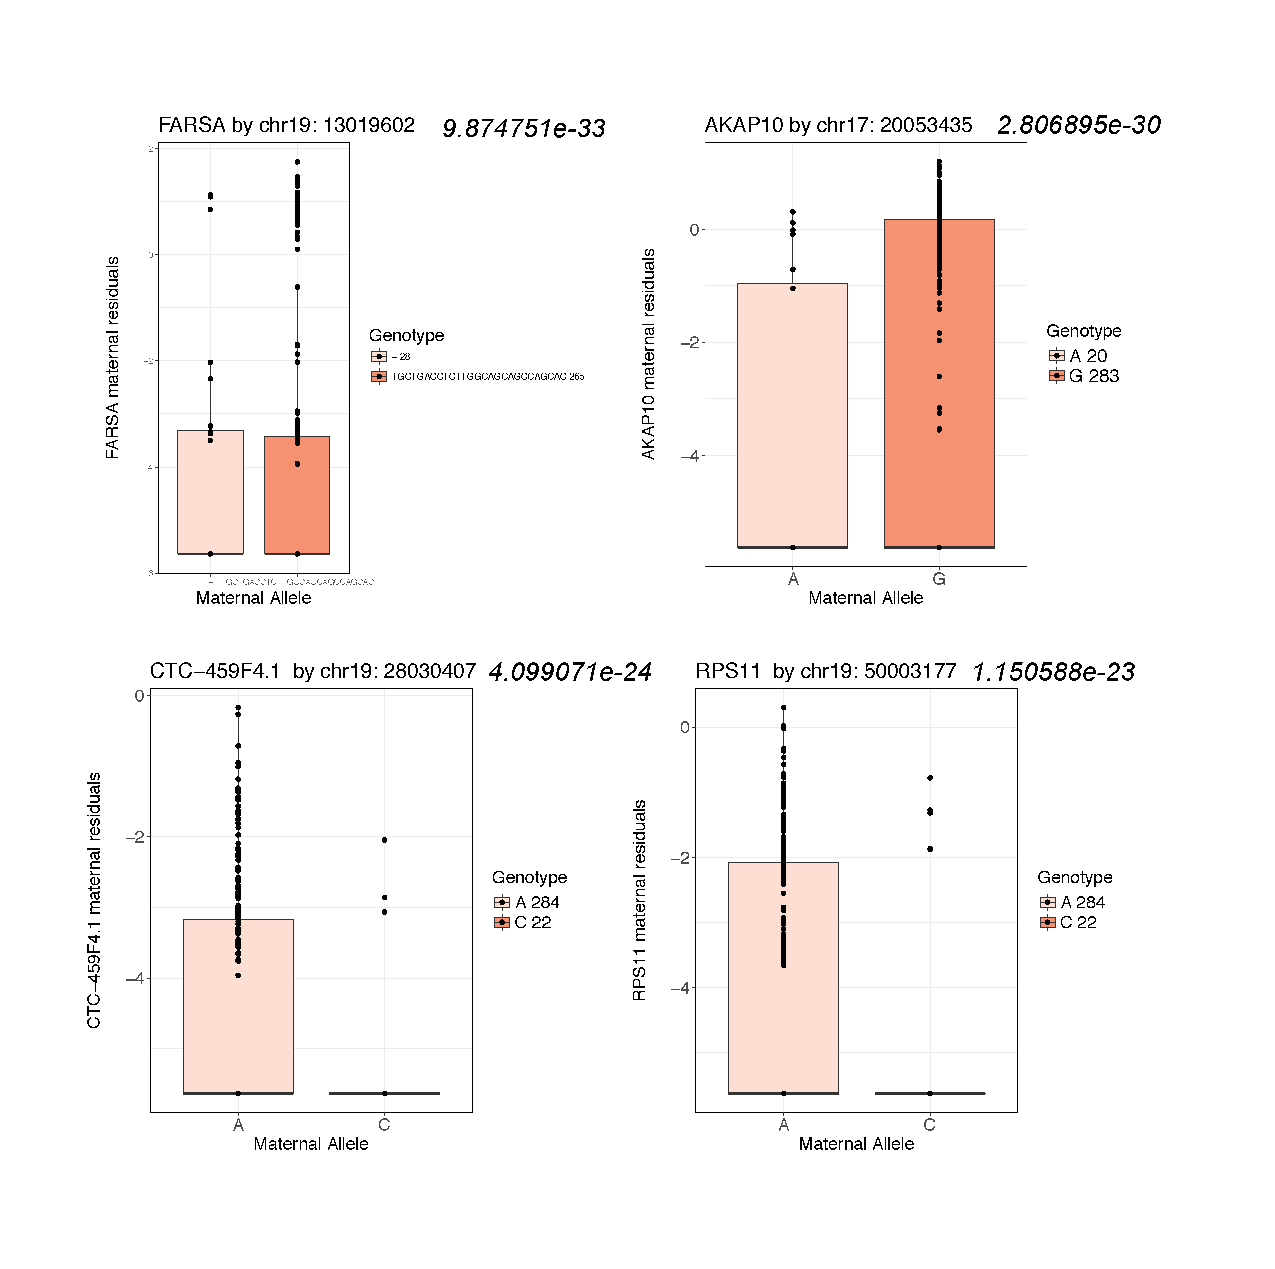
\includegraphics[width=4in]{img/ch04/fig-04-mat-eQTL.pdf}
\caption[Maternal eQTL Associations driven by zeros.]{\textbf{Maternal eQTL Associations driven by zeros.} }
\label{fig:mat-eQTL}
\end{figure}

\begin{figure}[!htb]
\centering 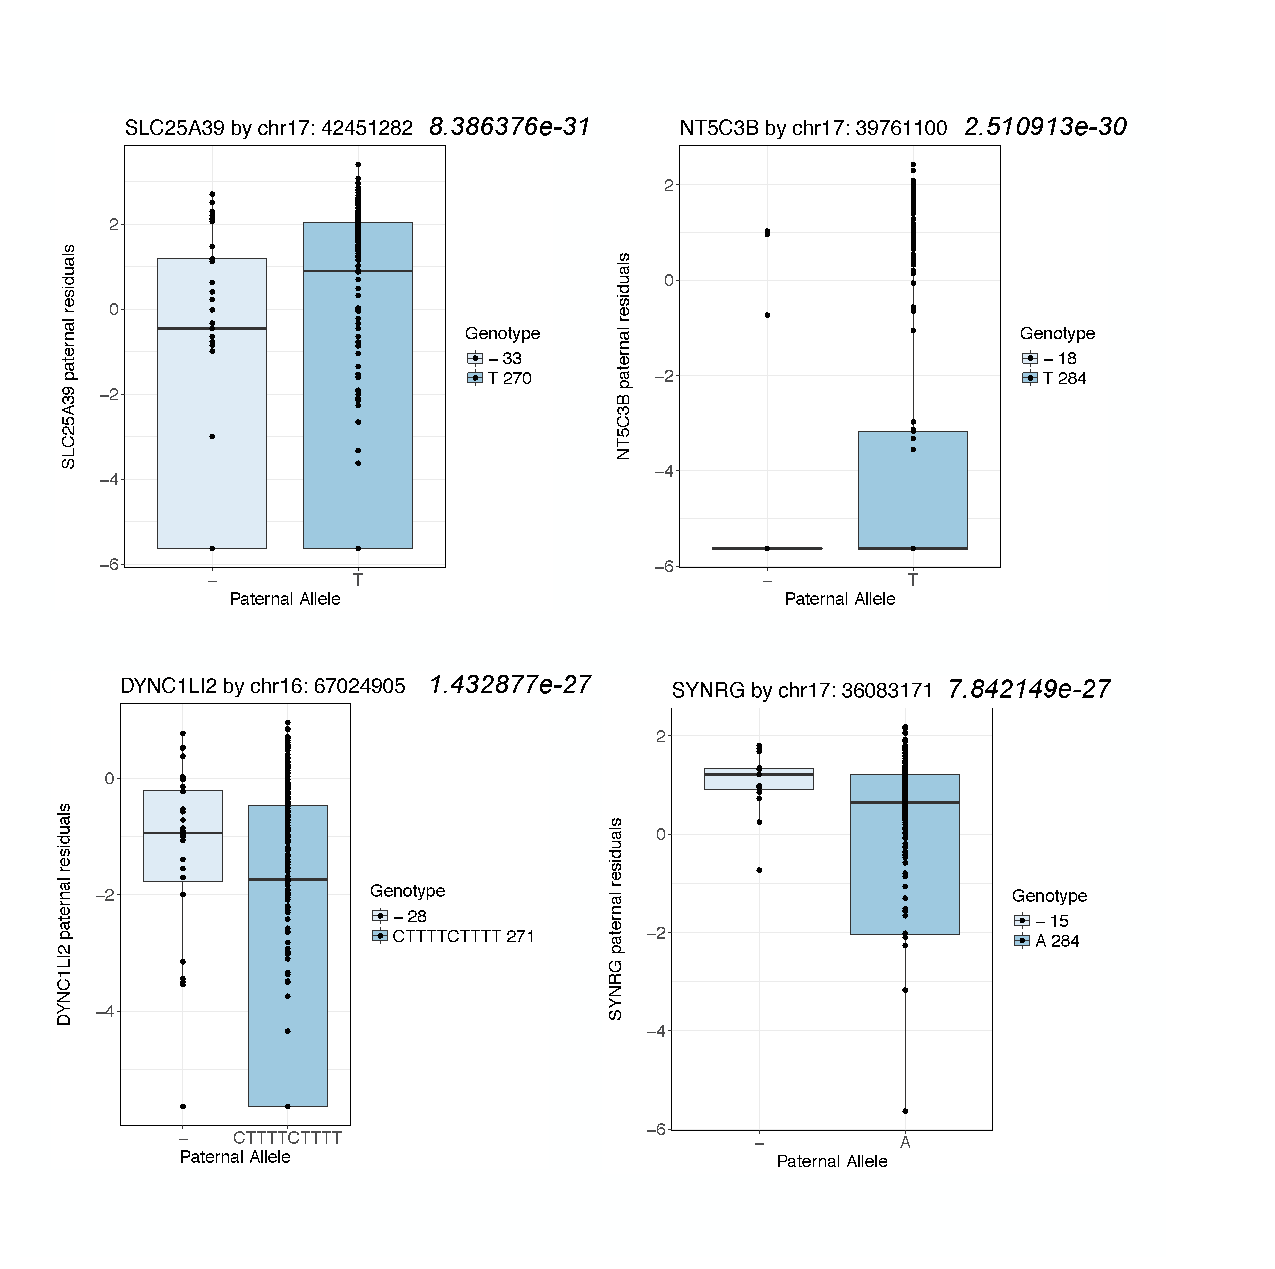
\includegraphics[width=4in]{img/ch04/fig-05-pat-eQTL.pdf}
\caption[Paternal eQTL Associations driven by zeros.]{\textbf{Paternal eQTL Associations driven by zeros.} }
\label{fig:pat-eQTL}
\end{figure}


I then redid the same analysis using informative reads, removing zeros that were due to absence of heterozygous SNPs in the gene. There were xx SNP gene pairs we could compare across both single parent eQTLs. For those significant in one or the other, the effect sizes were all in the same direction, no SNPs had opposite effects on their corresponding parental gene expression (Figure \ref{fig:effectsizes}). The imbalance of positive and negative effect sizes in Figure \ref{fig:effectsizes} is likely due in part to the zeros in the data where few genes have expression and drive the effect size to be positive.

\begin{figure}[!htb]
\centering \includegraphics[width=5in]{img/ch04/fig-06-effectsizes.pdf}
\caption[Similar effect sizes across mat-eQTL and pat-eQTL.]{\textbf{Similar effect sizes across mat-eQTL and pat-eQTL.} }
\label{fig:effectsizes}
\end{figure}


We then compared SNP gene pairs that were significant (Bonferroni) in one parent, and not significant (p \textgreater 0.05) in the other parent (7,712 SNP gene pairs were maternally significant and not paternally significant; 10,815 paternal significant associations not maternally significant). An example in Figure . 

\subsection{Modified ASE Test}\label{Modified ASE Test} 

To detect parent of origin effects on expression another way, we did a modified ASE test (see Methods) using parental gene expression count data. Using a Bonferonni corrected p-value we identified xx significant results. The top ten significant genes with their most significant SNPs are included in Table 1. The top three genes with their most significant SNPs shown in Figure \ref{fig:top3}. Of the first four significant genes, three were imprinted genes.


\begin{figure}[!htb]
\centering 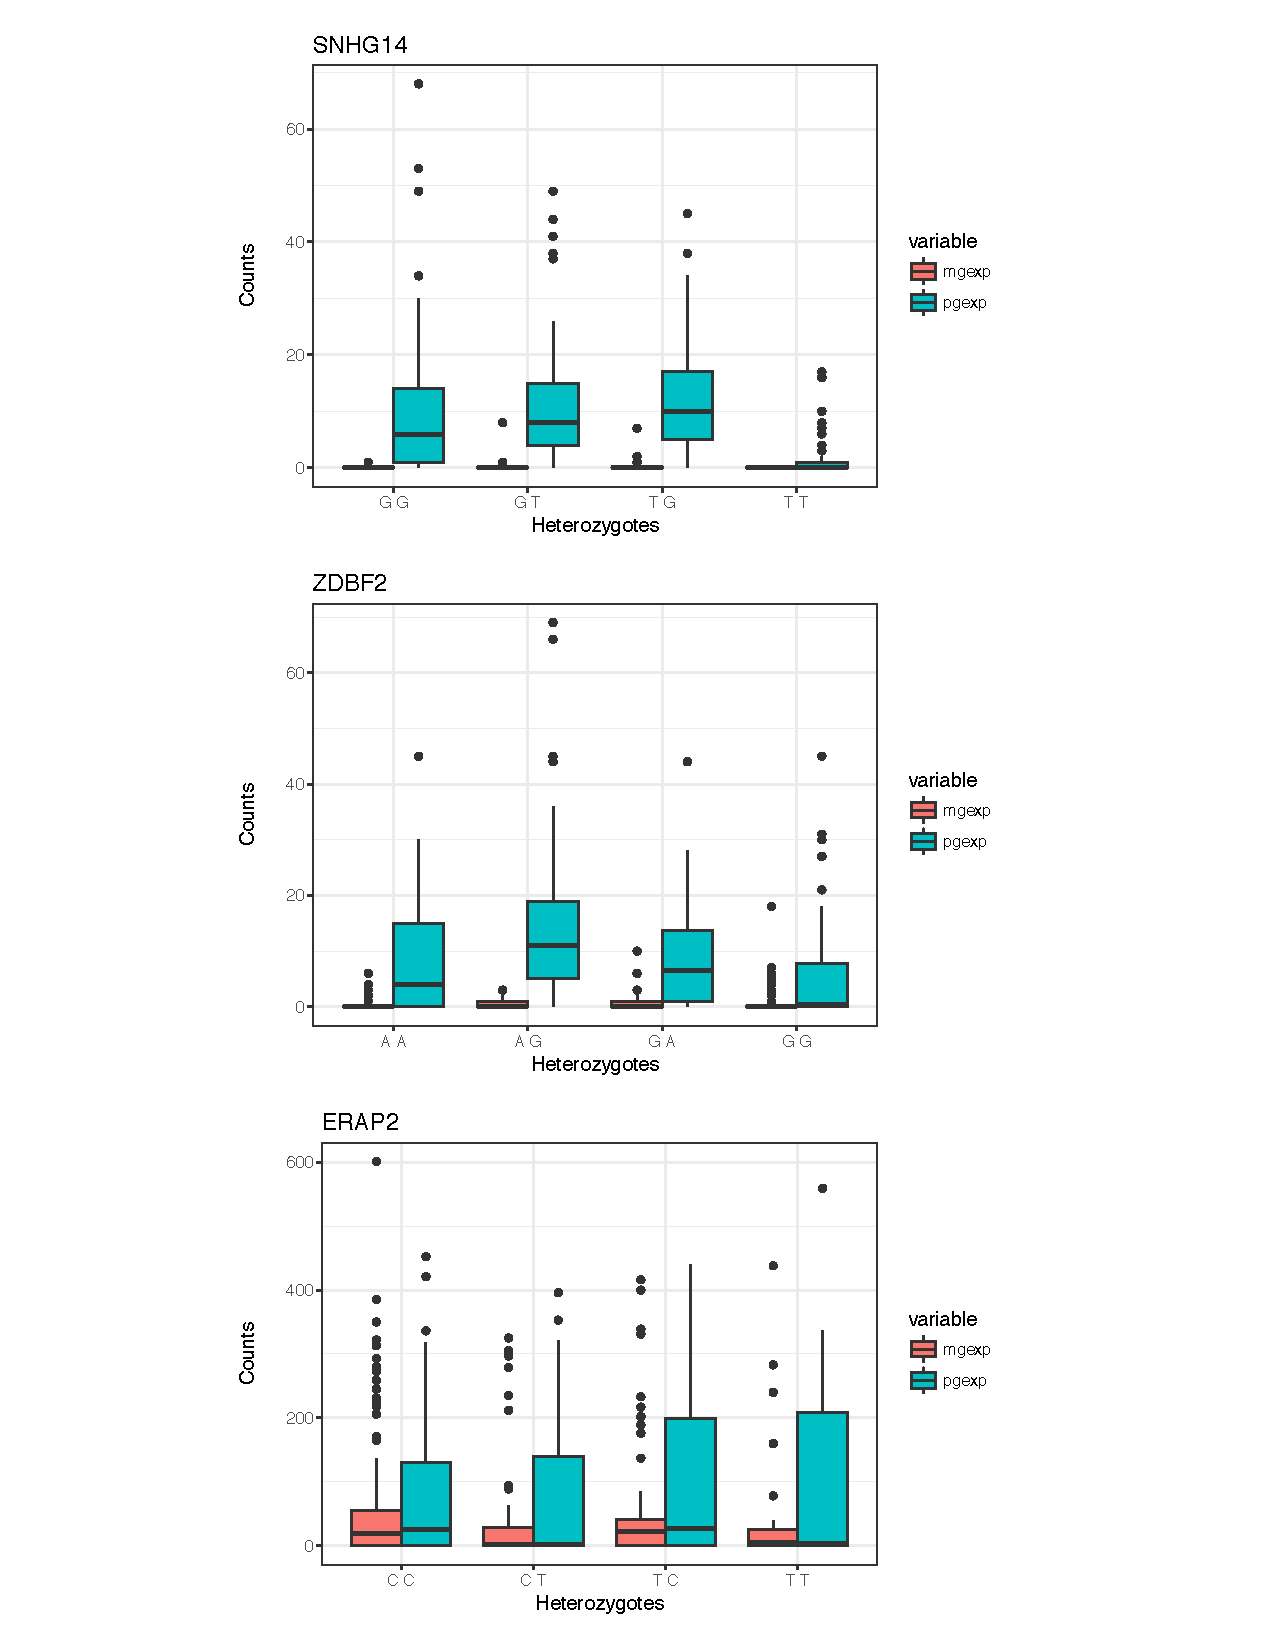
\includegraphics[width=5in]{img/ch04/fig-07-top3.pdf}
\caption[Top three significant genes from modified ASE test.]{\textbf{Top three significant genes from modified ASE test.} }
\label{fig:top3}
\end{figure}


\subsection{Modified ASE Test on Symmetrically Expressed Genes}\label{Modified ASE Test on Symmetrically Expressed Genes} 
To not include imprinted genes in the analysis we only tested genes that had symmetrical expression (see Methods). 



\section{Discussion}\label{ch04-discussion}

Previous studies using parental alleles and gene expression have identified imprinted genes and genetic variation that affects quantitative traits\cite{Zoledziewska:2015do,Baran:2015cx,Benonisdottir:2016dz,Garg2012a}, but none to our knowledge have looked at how genetic variation can impact parent of origin expression.

Here we used parental specific gene expression in 306 Hutterite individuals to characterize genetic variation on parental expression. We first performed a parent of origin opposite effect eQTL (oeQTL) using total gene expression. We then did a maternal and paternal eQTL on maternal and paternal gene expression (mat-eQTL, pat-eQTL), respectively. We finally looked for parent of origin effects among reciprocal heterozygotes.

Our opposite effect model has been successful in identifying opposite effects of parentally inherited variants on quantitative traits in the Hutterites but found none with LCL gene expression. These could be due to a number of limitations of this study, including sample size and tissue studied. Additionally we did our \emph{cis} mat-eQTL and pat-eQTL. This test identified known significant eQTLs as they would show up in both mat-eQTL and pat-eQTL results since standard eQTLs do not depend on the parent of origin. None of the variants compared across the two showed opposite effects by parent of origin. We were not able to find any maternal or paternally only effects on gene expression.

We found that most of the negative results were driven by sparsity in the data. Zeros in gene expression could be due to two factors: 1) no heterozygous/parent of origin SNPs in the gene such that homozygous reads could not be assigned to a parent, or 2) there are heterozygous SNPs in the genes but there are no reads. We assigned genes for individuals that did not have any heterozygous SNPs as missing and kept the values for those with at least one heterozygous site in a gene. This resulted in different numbers of individuals and genes to be tested. This provided a more conservative and informative data set but we did not find any significant maternal or paternal only effects on gene expression.

Finally, we performed a modified ASE test among reciprocal heterozygotes to identify effects of parental variation on gene expression. The missing gene expression (i.e. uninformative) for some individuals, decreased the numbers of reciprocal heterozygotes we could test for each gene.

These few results could be due to many limitations of our study. Although we were able to determine the parent of origin for many transcripts in the Hutterites, we could not assign every RNA sequencing read to a parent due to lack of heterozygous sites or missing parent of origin information for alleles. A lot of genes were missing parental gene expression resulting in very sparse data. Second, we conducted these studies in LCLs, and therefore could only study parent of origin effects in LCLs and would miss any effects in other tissues or developmental time points. Additionally, our models to test for parent of origin eQTL effects are decent but could be much improved, such as to model over-dispersion in gene expression.

In summary, we did not identify any genetic variation that has parent specific or opposite parental effects on parental specific or total gene expression.


\section{Methods}\label{ch04-methods}

\subsection{Genotypes and Sample Information}\label{Genotypes and Sample Information}
LCL RNA-seq transcripts for 306 individuals were mapped to parental haplotypes as in Chapter \ref{ch:imprinted}. We used the measures of total as well as maternal and paternal expression in this study. We used multiple approaches to characterize parent of origin effects on gene expression.
To be conservative, we used 306 Hutterite individuals for which we have parental genotypes and tested SNPs for which we have at least three individuals in at least three of four parent of origin genotype classes (such that we have at least three individuals in at least one heterozygote category and one heterozygote individual will not drive our analysis). We used QCed SNPs with MAF \textgreater 5\%.

\subsection{RNA-seq QC}\label{RNA-seq QC}
Multiple approaches required different QC method. For the total gene expression, we used normalized gene expression. First, we removed lowly expressed genes with a log count per million (cpm) greater than 1 in at least 20 individuals.The R/Bioconductor package edgeR was used to convert the RNA-seq counts to log2 TMM-normalized CPM values\cite{Robinson:2010dd,Robinson:2010cw}. Technical covariates correlated with gene expression Principal Components were regressed out (RIN, DNA concentration, RNA concentration, Flowcell/Lane). 

\subsection{Parent of Origin Expression QC}\label{Parent of Origin Expression QC}
Maternal gene expression was used as both counts and as normalized gene expression. Maternal gene expression counts were used directly from STAR gene count output\cite{Dobin:2002by} subsetted on genes included in the total gene expression analysis. 
Normalized maternal expression was calculated using similar to total gene expression using edgeR and converting RNA-seq counts to log2 TMM normalized CPM values using normalization factors (library sizes) from the total gene expression (maternal gene expression too sparse on it's own). 
Same method was used to get paternal gene expression counts and normalized paternal gene expression.

\subsection{Informative Genes}\label{Informative Genes}
To separate informative parental gene expression from uninformative parental gene expression I compiled all of the heterozygous SNPs for each individual for each gene that was expressed in LCLs. If a gene for an individual did not have any heterozygous parent of origin SNPs (i.e. informative SNPs), the gene was considered missing (converted to NA for downstream analysis). If there was at least one heterozygous parent of origin SNPs in the corresponding gene, the gene expression value was not altered, since zero expression for that gene for that parent could be informative. This nulled different numbers of genes for different individuals (Figure \ref{fig:indspergene}).

\begin{figure}[!htb]
\centering \includegraphics[width=5in]{img/ch04/fig-08-individualspergene.pdf}
\caption[Number of Individuals with Gene Expression.]{\textbf{Number of Individuals with Gene Expression.} }
\label{fig:indspergene}
\end{figure}



\subsection{Opposite Parent of Origin eQTL}\label{Opposite Parent of Origin eQTL}
We used the same method outlined in Chapter \ref{ch:pogwas} to detect if SNPs had opposite effects on total gene expression by parental origin. 

\subsection{Single Parent eQTL}\label{Single Parent eQTL}
To use the parent of origin expression, we performed a \emph{cis} eQTL testing for specific parental effects on the same parental gene expression as follows. We defined \emph{cis} as +/- 250kb from the TSS of the gene. 

\begin{equation}
Y _{M}=W\alpha + X_{M}\beta_{M}+g+\epsilon
\end{equation}

\begin{equation}
Y _{P}=W\alpha + X_{P}\beta_{P}+g+\epsilon
\end{equation}


\subsection{Modified ASE Test}\label{Modified ASE Test}
We used a simple $\chi^2$ test on the reciprocal heterozygotes on their corresponding maternal and paternal expression using maternal and paternal count data corresponding to haplotype specific expression. 


\subsection{Not asymmetrically expressed genes}\label{Not asymmetrically expressed genes}
We used a binomial test to determine genes that had more maternal expression than paternal expression. We summed gene expression across all individuals for a gene  We kept genes not significant (Bonferonni, p \textgreater 3.5e-06) and used those for the Modified ASE Test. 







% Format a LaTeX bibliography
\makebibliography

% Figures and tables, if you decide to leave them to the end
%\input{figure}
%\input{table}

\end{document}


